\chapter{Results} \label{chap:results}

This chapter presents and analyzes the empirical findings from our experiments.
We review the pre-training performance of \ChristBERT{} variants as well as
their downstream task performance alongside other domain-specific and general
language models. The results provide insights into model effectiveness across
named entity recognition and text classification tasks in the medical domain.

\section{Pre-Training Performance}

Fig.~\ref{fig:ppl} plots the perplexity of the three \ChristBERT{} models during
pre-training over 100,000 training steps. Perplexity was evaluated on a held-out
validation set of 3,000 randomly chosen documents from our pre-training corpus
listed in Tab.~\ref{tab:corpus_stats}. We observe that the different domain
adaptation strategies are reflected in the perplexity trajectories in terms of
initial perplexity, rate of decline and convergence behavior. 

\begin{figure}[htbp]
  % \begin{subfigure}{0.95\textwidth}
  %   \centering
  %   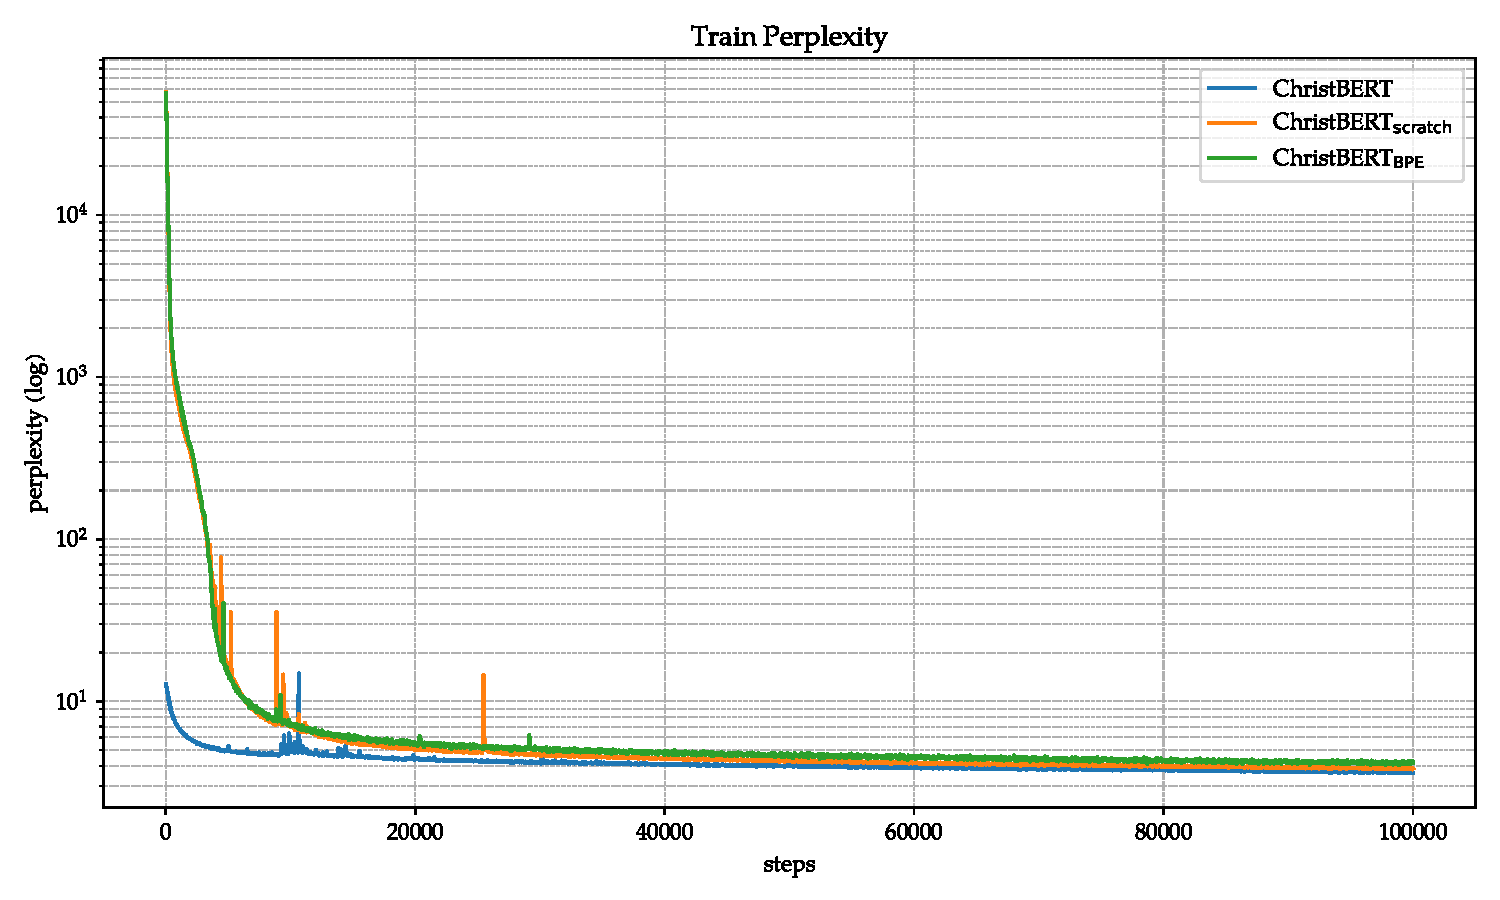
\includegraphics[width=\textwidth]{ppl_train}
  %   \caption{Perplexity on training set}
  % \end{subfigure}
  % \begin{subfigure}{0.95\textwidth}
  %   \centering
  %   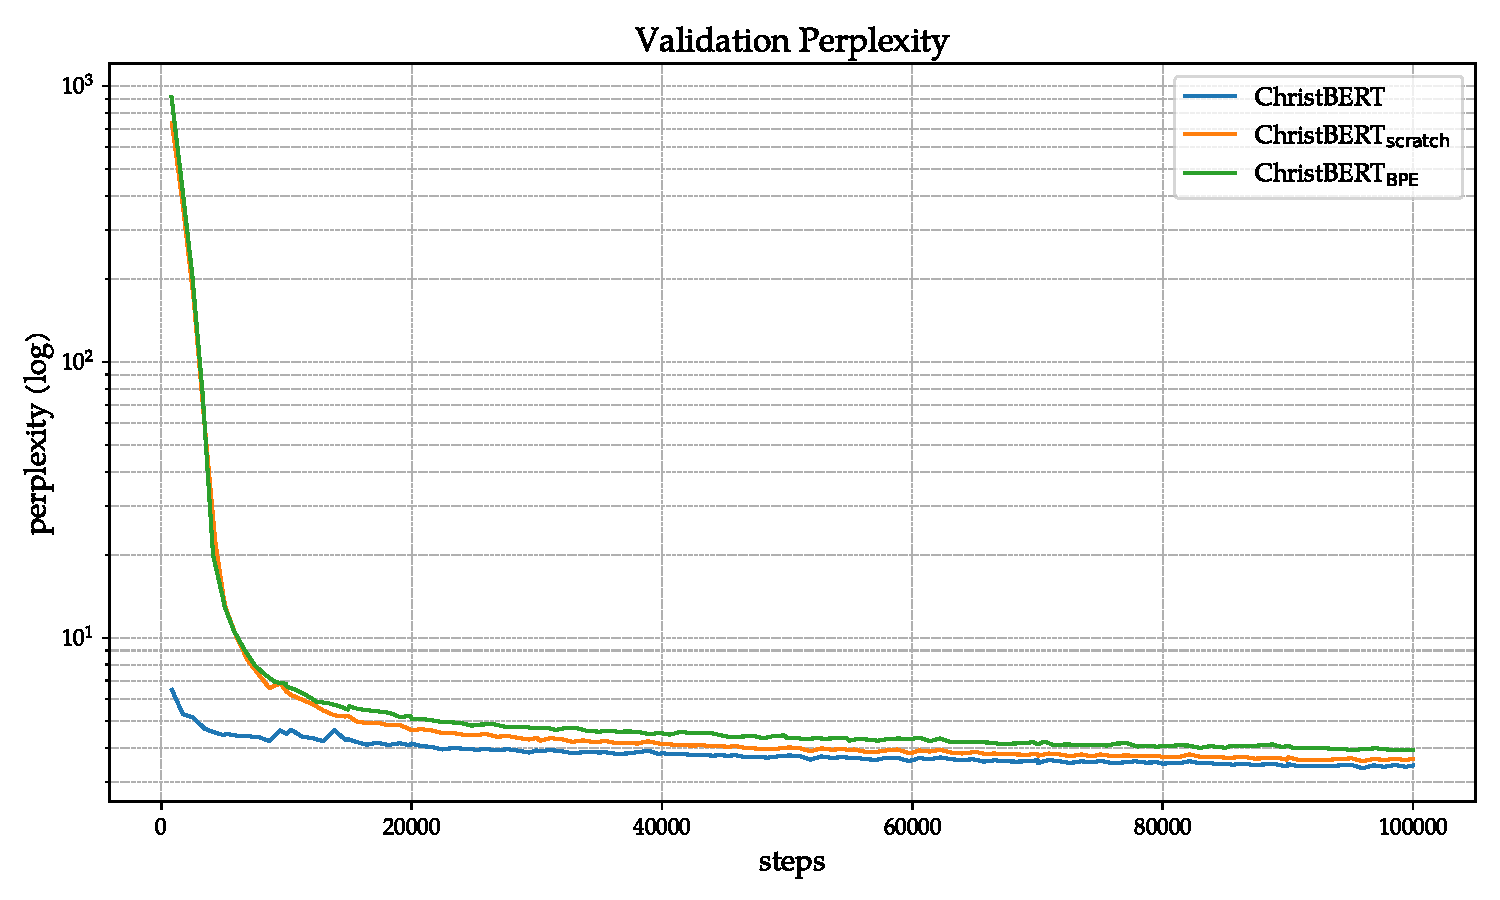
\includegraphics[width=\textwidth]{ppl_val}
  %   \caption{Perplexity on validation set}
  % \end{subfigure}
  \centering
  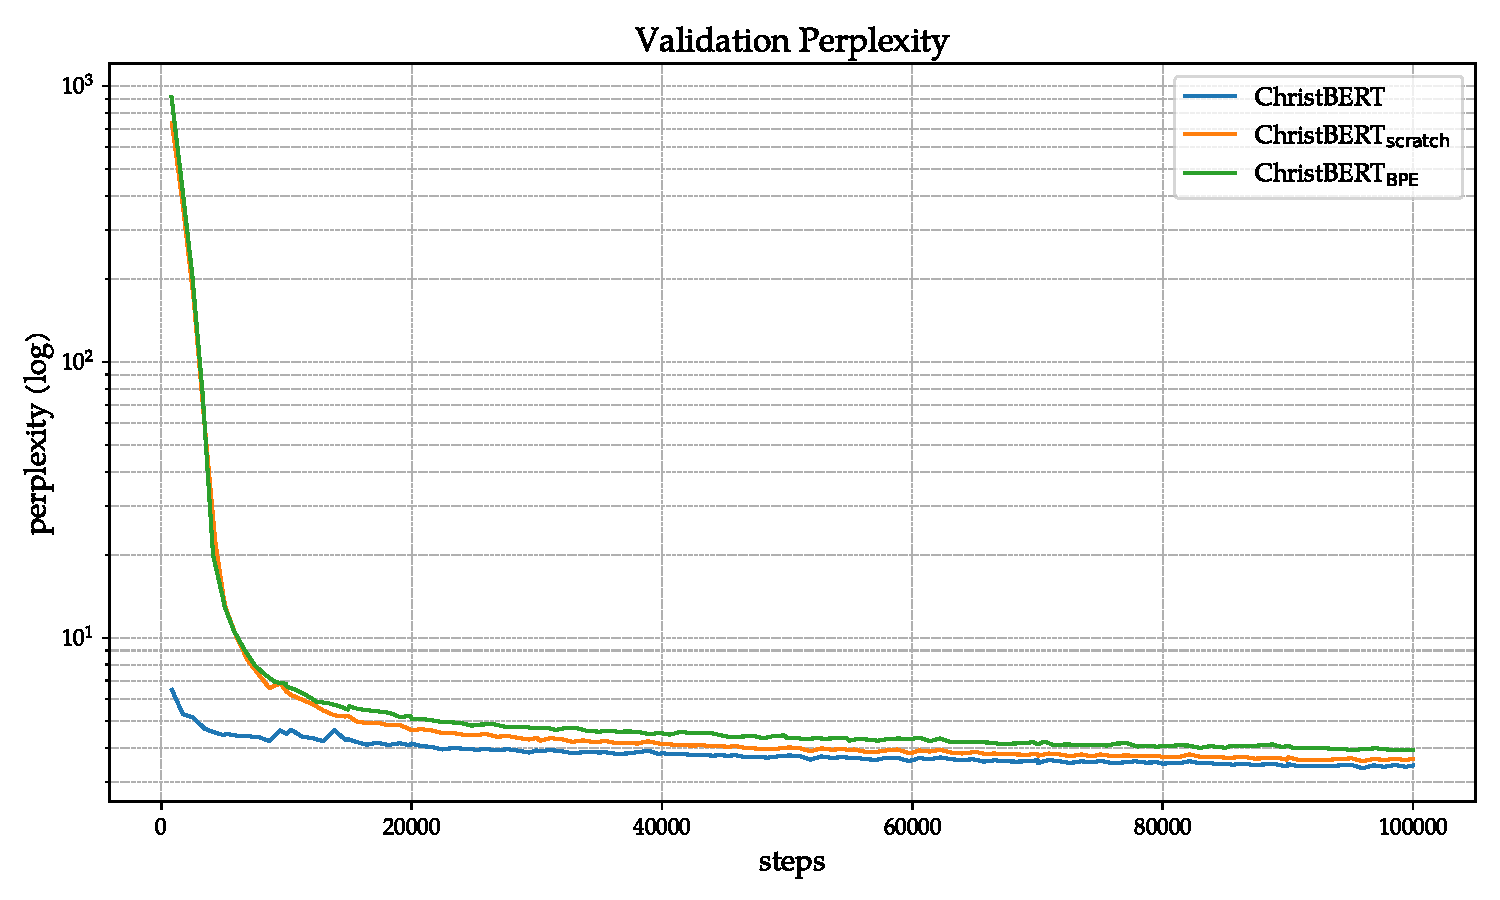
\includegraphics[width=0.95\textwidth]{ppl_val}
  \caption[Perplexity during pre-training of \ChristBERT{} models]{Perplexity
  during pre-training of \ChristBERT{} models. Perplexity is shown in log scale
  for every optimization step and evaluated on the validation split
  of the pre-training corpus.}
  \label{fig:ppl}
\end{figure}

\subsubsection{Initial Perplexity and Rate of Decline}
Initially, the two \ChristBERT{} variants pre-trained from scratch exhibit high
perplexity values of $57434.5$ and $56343.3$, while the continuously pre-trained
\ChristBERT{} starts with a lower perplexity of $12.64$. The lower perplexity
directly results from the model being initialized with the weights of GeistBERT,
demonstrating the effectiveness of transfer learning. As pre-training
progresses, perplexity decreases steeply during the first 10,000 steps for
\ChristBERT\textsubscript{scratch} and \ChristBERT\textsubscript{BPE}, with the
rate of perplexity reduction following a non-linear pattern across all variants.
The steepest reduction occurs within the first 5,000 steps, where we observe
perplexity values dropping approximately two orders of magnitude from ${\sim}
10^3$ to ${\sim} 10^1$. The observed perplexity curve can be attributed to the
learning rate schedule, in which the learning rate is linearly increased for
10,000 iterations to its maximum. After this warmup phase, the perplexity
trajectory flattens considerably between steps 10,000 and 40,000. Model
perplexity continues to decrease but at a substantially slower rate, which is
due to the learning rate following a polynomial decay to zero after the first
10,000 steps.

\subsubsection{Convergence Behavior}
The continuously pre-trained \ChristBERT{} model converges the fastest,
stabilizing at around a perplexity of 3-4 by 10,000 steps and maintaining the
lowest perplexity throughout pre-training. Additionally, \ChristBERT{}
consistently achieved lower perplexity than both BPE and Scratch variants, with
perplexity values 30-50\% lower during the middle stages of pre-training.
Despite this, after around 40,000-50,000 iterations, all models reach a
relatively stable perplexity level between 2-4. Diminishing returns are observed
after 60,000 steps, suggesting extended pre-training offers minimal improvements
and convergence is achieved. Moreover, we observed divergence in some
pre-training runs, particularly due to high learning rates where model
parameters were updated too aggressively. This divergence manifested as sudden
spikes in perplexity and subsequent failure to converge as shown in
Fig.~\ref{fig:div_ppl} in the Appendix. To mitigate this, we found that lowering
the learning rate was effective in stabilizing pre-training. This was necessary
for \ChristBERT\textsubscript{scratch} and \ChristBERT\textsubscript{BPE}, where
we reduced the maximum learning rate from \num{7e-4} to \num{6e-4}, while with
the GeistBERT initialization it was possible to use a higher peak learning rate.
\\

\ChristBERT\textsubscript{BPE} consistently demonstrates the highest perplexity
values among the three variants, particularly in the middle stages of
pre-training. This effect likely stems from its custom byte-pair
encoding vocabulary, where it spends the middle stages learning different
language representations. As discussed in Sec.~\ref{sec:lm_eval}, perplexity
comparisons are most meaningful between models sharing the same tokenizer,
therefore this difference does not necessarily indicate inferior model quality.
Furthermore, an improvement in an intrinsic measure such as perplexity does not
necessarily correlate with enhanced performance in extrinsic measures such as
practical downstream language tasks. However, as a measure of the LM's
generalization capabilities, it is still a useful indicator of its potential
performance on downstream tasks, which we will analyze in the following
sections.

\section{Fine-Tuning Performance}

\subsection{Named Entity Recognition}

Tab.~\ref{tab:eval_ner_metrics} shows the performance results of medical
named entity recognition on the BRONCO150, CARDIO:DE and GGPONC datasets.
Detailed results for each entity type in the respective dataset are reported in
Tab.~\labelcref{tab:bronco,tab:cardiode,tab:ggponc2} in the Appendix. The
\ChristBERT{} models consistently outperform the baseline models across all
datasets, establishing a new state-of-the-art German biomedical NER.

\begin{table}[htbp]
    \centering
    % Prompt: Fill in the values in the tex table. The column for the column values in the csv is predict_micro_[precision, recall, f1]. Format the values in percent without the symbols i.e. xx.xx. The values belong in the tex table with row model_name and column data_name.

\begin{tabular}{l ccc ccc ccc}
    \toprule
    \multirow{2}{*}[-0.5\dimexpr \aboverulesep + \belowrulesep + \cmidrulewidth]{\bfseries Model} &
    \multicolumn{3}{c}{\bfseries BRONCO150} &
    \multicolumn{3}{c}{\bfseries CARDIO:DE} &
    \multicolumn{3}{c}{\bfseries GGPONC} \\
    \cmidrule(lr){2-4} \cmidrule(lr){5-7} \cmidrule(lr){8-10}
    & Prec. & Rec. & \ff &
    Prec. & Rec. & \ff &
    Prec. & Rec. & \ff \\
    \midrule
     \ChristBERT & 81.42 & 81.77 & 81.87 & 85.58 & 89.65 & 87.57 & 75.65 & \textbf{79.83} & \textbf{77.69} \\
     \ChristBERT\textsubscript{scratch} & \underline{81.87} & \underline{82.32} & \underline{82.09} & 88.38 & 89.89 & 89.13 & \underline{76.54} & \underline{77.56} & \underline{77.05} \\
     \ChristBERT\textsubscript{BPE} & \textbf{85.71} & \textbf{83.78} & \textbf{84.74} & \underline{89.50} & \textbf{91.31} & \textbf{90.40} & \textbf{76.59} & 77.42 & 77.00 \\
     medBERT.de & 78.67 & 79.58 & 79.12 & 87.66 & 90.02 & 88.83 & 73.89 & 75.78 & 74.73 \\
     BioGottBERT & 76.96 & 78.45 & 77.70 & 88.37 & \underline{90.74} & 89.54 & 75.24 & 75.40 & 75.32 \\ 
     GeistBERT & 75.65 & 79.83 & 77.69 & 85.58 & 89.65 & 87.57 & 74.57 & 75.36 & 74.96 \\
     GeBERTa & 78.67 & 79.58 & 79.12 & \textbf{90.51} & 90.23 & \underline{90.37} & 75.96 & 76.93 & 76.45 \\
    \bottomrule
\end{tabular}
 
    \caption[Overview of micro averaged precision, recall and \ff{} scores
    achieved on the NER tasks]{Overview of micro averaged precision (Prec.),
    recall (Rec.) and \ff{} scores on the NER tasks. All results are shown in
    percent and assess each model's best fine-tuned performance on each
    downstream task's test set. The best model was selected out of 28 runs based
    on its validation set performance. Best score in bold and second best
    underlined.}
    \label{tab:eval_ner_metrics}
\end{table}

% \subsubsection{Per Dataset Performance Analysis}
On the BRONCO150 dataset, \ChristBERT\textsubscript{BPE} achieves the highest
precision (85.71\%), recall (82.32\%) and \ff{} score (84.74\%), forming a
substantial improvement over both specialized medical models and general
language models. \ChristBERT\textsubscript{scratch} places second with an \ff{}
of 83.33\%, followed closely by \ChristBERT{} with 81.87\%. The performance
delta between \ChristBERT{} variants and other models is particularly evident
when comparing against the general language models. For instance, the \ff{}
score of \ChristBERT\textsubscript{BPE} with 84.74\% represents a 5.62
percentage point improvement over GeistBERT (77.69\%) and a 5.08 percentage
point improvement over GeBERTa (79.12\%). This significant performance gap
underscores the value of domain-specific pre-training for NER in medical texts.

The performance on the CARDIO:DE dataset presents a different pattern of
results. Here, all compared models showed more similar performances, with
\ChristBERT\textsubscript{BPE} performing the best, followed closely by GeBERTa,
which leads among the baselines and demonstrates on par NER efficacy. Both
mentioned models achieve high \ff{} scores of 90.40\% and 90.37\%, respectively,
differing in precision and recall. This dataset highlights the potential for
general language models to perform competitively in certain medical subdomains
when trained appropriately.

The GGPONC dataset presents the most challenging evaluation scenario with eight
fine-grained semantic classes and long entity spans across a large corpus of
oncology documentation. On this complex dataset, \ChristBERT{} models again
demonstrate superior performance compared to the baseline models, with
\ChristBERT{} achieving the highest recall (79.83\%), while
\ChristBERT\textsubscript{BPE} attains the highest precision (76.59\%). Here,
\ChristBERT\textsubscript{BPE} and \ChristBERT\textsubscript{scratch} match each
other's precision, recall and \ff{} scores. The performance advantage of our
pre-training corpus on GGPONC is particularly noteworthy given the complexity of
this dataset. With an \ff{} of 77.69\%, \ChristBERT{} is the best performing NER
model and outperforms the next best non-\ChristBERT{} model GeBERTa at 76.45\%
by 1.24 percentage points. The demonstrated advantage in the most complex
dataset suggests that the domain-specific pre-training of \ChristBERT{} models
enables more effective learning of the nuanced entity boundaries and semantic
distinctions required for fine-grained medical entity recognition.

\subsubsection{Cross-Model Analysis and Domain Specialization Effects}
Among the \ChristBERT{} variants, \ChristBERT\textsubscript{BPE} consistently
demonstrates strong performance across all NER datasets, achieving the highest
or second-highest \ff{} scores in each experiment. This suggests that the custom
BPE vocabulary approach may offer advantages for handling the morphological
complexity and specialized vocabulary found in German medical texts. Despite its
seemingly weaker performance during pre-training as indicated by higher
perplexity values, its downstream performance confirms that pre-training metrics
do not necessarily translate into task-specific effectiveness.

\ChristBERT\textsubscript{scratch} also performs competitively across NER
datasets, indicating that domain-specific training from initialization can be
effective without leveraging transfer learning from general domain pre-training.
The continuously pre-trained \ChristBERT{} model shows particular strength in
the GGPONC dataset, suggesting it may have advantages for handling complex,
fine-grained entity recognition tasks.

The comparison between specialized medical models (\ChristBERT{} variants,
medBERT.de, BioGottBERT) and general language models (GeistBERT, GeBERTa)
reveals distinct performance behavior in medical NER. In BRONCO150 and GGPONC,
domain-specific models generally outperform general models, confirming the value
of specialized pre-training for oncology text. However, in CARDIO:DE, GeBERTa
achieves the highest \ff, suggesting that general language models can be
competitive in certain medical subdomains when trained on heterogeneous and
cross-domain data. Notably, 8\% of GeBERTa’s pre-training data consisted of
medical texts. 

This variability illustrates that domain specificity presents different
advantages depending on the particular medical subdomain and entity types being
targeted. The general language models appear more competitive on CARDIO:DE,
possibly due to differences in writing style, terminology standardization, or
entity class definitions between cardiovascular and oncology domains.
Interestingly, we observe GeistBERT exhibiting equivalent performance to the
domain-adapted model BioGottBERT. We attribute this mainly to the relatively
small size of BioGottBERT's biomedical training corpus (0.8 GB), highlighting
the importance of corpus size in achieving effective domain adaptation.

An analysis of precision and recall values reveals different optimization
patterns across models. \ChristBERT\textsubscript{BPE} tends to favor precision
over recall in BRONCO150 and GGPONC, while achieving high values in both metrics
for CARDIO:DE. In contrast, the continuously pre-trained \ChristBERT{} shows
stronger recall performance, particularly in GGPONC. These trade-offs have
important implications for clinical applications, where the relative importance
of precision versus recall may vary based on the specific use case.
\subsection{Text Classification}

Tab.~\ref{tab:eval_cls_metrics} presents the classification results for each
model on the CLEF and JSynCC classification datasets. Detailed results for each
topic category in JSynCC can be found in Tab.~\ref{tab:jsyncc} in the Appendix.
We omit a separate per class drill-down for the CLEF dataset as it contains over
230 classes. As such, the CLEF benchmark poses the more challenging multi-label
classification task, while JSynCC only requires assigning labels out of six
medical categories.

\begin{table}[htbp]
    \centering
    % Prompt: Fill in the values in the tex table. The column for the column values in the csv is predict_micro_[precision, recall, f1]. Format the values in percent without the symbols i.e. xx.xx. The values belong in the tex table with row model_name and column data_name.

\begin{tabular}{l ccc ccc}
    \toprule
    \multirow{2}{*}[-0.5\dimexpr \aboverulesep + \belowrulesep + \cmidrulewidth]{\bfseries Model} &
    \multicolumn{3}{c}{\bfseries CLEF} &
    \multicolumn{3}{c}{\bfseries JSynCC} \\
    \cmidrule(lr){2-4} \cmidrule(lr){5-7} 
    & Prec. & Rec. & \ff & 
    Prec. & Rec. & \ff \\
    \midrule
    \ChristBERT & 78.12 & 75.34 & 76.03 & 89.01 & \textbf{100} & \underline{94.19} \\
    \ChristBERT\textsubscript{scratch} & \textbf{93.68} & 85.17 & \underline{89.22} & \underline{91.86} & 97.53 & \textbf{94.61} \\
    \ChristBERT\textsubscript{BPE} & 88.22 & \underline{88.35} & 88.28 & 89.53 & 95.06 & 92.22 \\
    medBERT.de & 89.21 & 87.59 & 88.40 & 91.25 & 90.12 & 90.68 \\
    BioGottBERT & 88.30 & 87.90 & 88.10 & 88.89 & \underline{98.77} & 93.57 \\
    GeistBERT & \underline{90.43} & 72.92 & 80.74 & \textbf{92.59} & 92.59 & 92.59 \\
    GeBERTa & 88.91 & \textbf{89.71} & \textbf{89.31} & \textbf{92.59} & 92.59 & 92.59 \\
    \bottomrule
\end{tabular}
 
    \caption[Overview of micro averaged precision, recall and \ff{} scores
    achieved on the classification tasks]{Overview of micro averaged precision
    (Prec.), recall (Rec.) and \ff{} scores on the classification tasks. All
    results are shown in percent and assess each model's best fine-tuned
    performance on each downstream task's test set. The best model was selected
    out of 28 runs based on its validation set performance. Best score in bold
    and second best underlined.}
    \label{tab:eval_cls_metrics}
\end{table}

On the CLEF dataset, GeBERTa achieves the highest \ff{} score at 89.31\%, driven
by its superior recall at 89.71\%. Nonetheless,
\ChristBERT\textsubscript{scratch} demonstrates the highest precision (93.68\%),
indicating that it is more effective at minimizing false positives. However, its
recall (85.17\%) is lower than GeBERTa's, resulting in a lower overall \ff{} at
89.22\%. To our surprise, we observe that both general and domain-specific
models perform similarly on this dataset. Notably, the continuously pre-trained
\ChristBERT{} variant shows the lowest overall performance among the evaluated
models on this dataset with an \ff{} of 76.03\%. Its performance differs by 4.61
percentage points from the next best model GeistBERT (80.64\%), its general
domain counterpart. This suggests that the continuous pre-training approach may
not be as effective for complex multi-label classification problems,
particularly when compared to the other \ChristBERT{} variants, which were
pre-trained with the same corpus but with different initialization strategies. 

It should be noted that GeBERTa included CLEF data in its pre-training corpus,
meaning it had already seen this data before evaluation. This data leakage
significantly undermines the validity of GeBERTa's performance metrics on this
specific dataset, as the model had prior exposure to the test data. This might
explain its exceptionally high performance compared to other models and should
be considered when interpreting these results. Even so, medBERT.de achieves
strong performance with an \ff{} score of 88.40\%, demonstrating that domain
adaptation across different medical subdomains supports the processing of
specialized terminology and concepts in animal experiment documentation.

On the JSynCC dataset, the majority of \ChristBERT{} models considerably
outperform the baseline models, with \ChristBERT\textsubscript{scratch}
achieving the highest \ff{} score of 94.61\%, closely followed by \ChristBERT{}
at 94.19\% and a shared third place between GeistBERT and GeBERTa at 92.59\%. A
particularly striking observation is the perfect recall (100\%) of \ChristBERT{}
on the JSynCC dataset, indicating that it identifies all relevant specialty
classifications across the test documents. However, its precision (89.01\%) is
lower than other models, resulting in an \ff{} of 94.19\%. This pattern suggests
that \ChristBERT{} may be over-predicting certain class labels, but its
comprehensive coverage ensures no relevant classifications are missed, a
characteristic that could be valuable in clinical applications where missing a
relevant specialty category might have significant consequences. 

The performance clustering on JSynCC is notably tight, with all models achieving
\ff{} scores between 92.59\% and 94.61\%. Notably, BioGottBERT achieves the
second-highest overall performance on JSynCC with an \ff{} of 93.57\% and recall
of 98.77\%. This suggests that the synthetic nature of this corpus may present
more standardized linguistic patterns that various model architectures can
effectively learn during fine-tuning. Furthermore, while
\ChristBERT\textsubscript{BPE} has consistently shown the best performance in
NER tasks, it does not rank among the top models on all classification
benchmarks. This indicates that the BPE vocabulary may not be as effective for
text classification tasks, where the model's ability to generalize across
different contexts and semantic meanings is crucial.
